\documentclass{beamer}
\usetheme{Madrid}
\usepackage{listings}
%\usecolortheme{seahorse}
%Information to be included in the title page:
\title{Optimizations Assignment 2}
\author{Alexander Sepelenco, Niall Sauvage}
\date{2023}

\begin{document}

\frame{\titlepage}

\begin{frame}[fragile]
\frametitle{A look into the development process}
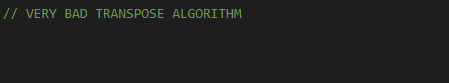
\includegraphics[width=1\textwidth]{images/opening_slide_joke1}
\end{frame}

\begin{frame}[fragile]
\frametitle{A look into the development process}
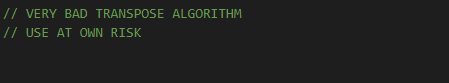
\includegraphics[width=1\textwidth]{images/opening_slide_joke2}
\end{frame}

\begin{frame}[fragile]
\frametitle{A look into the development process}
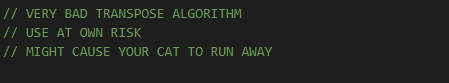
\includegraphics[width=1\textwidth]{images/opening_slide_joke3}
\end{frame}

\begin{frame}[fragile]
\frametitle{A look into the development process}
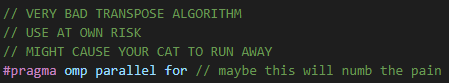
\includegraphics[width=1\textwidth]{images/opening_slide_joke4}
\end{frame}

\begin{frame}[fragile]
\frametitle{Bad Spatial Locality}
number of channels: 32..2048 (always powers of 2) \\
kernel order: 1, 3, 5, or 7
\begin{lstlisting}[language=C,keywordstyle=\color{blue}]
for ( c = 0; c < nchannels; c++ ) {
  for ( x = 0; x < kernel_order; x++) {
    for ( y = 0; y < kernel_order; y++ ) {
      sum += image[w+x][h+y][c] * kernels[m][c][x][y];
    }
  }
  output[m][w][h] = (float) sum;
}
\end{lstlisting}
\end{frame}

\begin{frame}[fragile]
\frametitle{Better Spatial Locality}
number of channels: 32..2048 (always powers of 2) \\
kernel order: 1, 3, 5, or 7
\begin{lstlisting}[language=C,keywordstyle=\color{blue}]
for ( x = 0; x < kernel_order; x++) {
  for ( y = 0; y < kernel_order; y++ ) {
    for ( c = 0; c < nchannels; c++ ) {
      sum += image[w+x][h+y][c] * kernels[m][c][x][y];
    }
  }
  output[m][w][h] = (float) sum;
}
\end{lstlisting}
\end{frame}

\begin{frame}[fragile]
\frametitle{First Look At Loop unrolling}
We can loop unroll our inner loop since nchannels can be big
\begin{lstlisting}[language=C,keywordstyle=\color{blue}]
for ( x = 0; x < kernel_order; x++) {
  for ( y = 0; y < kernel_order; y++ ) {
    for ( c = 0; c < nchannels; c+=4) { // power of 2 
      sum+=image[w+x][h+y][c]*kernels[m][c][x][y];
      sum+=image[w+x][h+y][c+1]*kernels[m][c+1][x][y];
      sum+=image[w+x][h+y][c+2]*kernels[m][c+2][x][y];
      sum+=image[w+x][h+y][c+3]*kernels[m][c+3][x][y];
    }
  }
  output[m][w][h] = (float) sum;
}
\end{lstlisting}
\end{frame}

\begin{frame}[fragile]
\frametitle{More Loop unrolling}
\begin{lstlisting}[language=C,keywordstyle=\color{blue}]
for ( x = 0; x < kernel_order; x++) {
  for ( y = 0; y < kernel_order; y++ ) {
    for ( c = 0; c < nchannels; c+=8) {
      sum+=image[w+x][h+y][c]*kernels[m][c][x][y];
      sum+=image[w+x][h+y][c+1]*kernels[m][c+1][x][y];
      sum+=image[w+x][h+y][c+2]*kernels[m][c+2][x][y];
      sum+=image[w+x][h+y][c+3]*kernels[m][c+3][x][y];
      sum+=image[w+x][h+y][c+4]*kernels[m][c+4][x][y];
      sum+=image[w+x][h+y][c+5]*kernels[m][c+5][x][y];
      sum+=image[w+x][h+y][c+6]*kernels[m][c+6][x][y];
      sum+=image[w+x][h+y][c+7]*kernels[m][c+7][x][y];
    }
  }
  output[m][w][h] = (float) sum;
}
\end{lstlisting}
\end{frame}

\begin{frame}[fragile]
\frametitle{Even More Loop unrolling}
\begin{lstlisting}[language=C,keywordstyle=\color{blue}]
for ( x = 0; x < kernel_order; x++) {
  for ( y = 0; y < kernel_order; y++ ) {
    for ( c = 0; c < nchannels; c+=16) {
      sum+=image[w+x][h+y][c]*kernels[m][c][x][y];
      sum+=image[w+x][h+y][c+1]*kernels[m][c+1][x][y];
      // 14 more times incrementing c index
    }
  }
  output[m][w][h] = (float)sum;
}
\end{lstlisting}
\end{frame}

\begin{frame}[fragile]
\frametitle{1D Arrays}
Every array will be return in 1D notation 
\begin{lstlisting}[language=C,keywordstyle=\color{blue}]
for ( x = 0; x < kernel_order; x++) {
  for ( y = 0; y < kernel_order; y++) {
    for ( c = 0; c < nchannels; c+=16) {
      int image_offset = (w+x) * width_offset + 
        ((h+y) * nchannels) + c;
      int kernel_total_offset = 
        m * kernel_offset + 
        x * kernel_order + y + c * ko2;
      sum += image_1d[image_offset] * 
        kernel[kernel_total_offset];
      sum += image_1d[image_offset + 1] * 
        kernel[kernel_total_offset + ko2 * 1];
    }
  }
}
\end{lstlisting}
\end{frame}

\begin{frame}[fragile]
\frametitle{Kernel Not In Contigous Memory}
kernel isn't accessed in contiguous memory
\begin{lstlisting}[language=C,keywordstyle=\color{blue}]
sum += image_1d[image_offset] * 
  kernel[kernel_total_offset];
sum += image_1d[image_offset + 1] * 
  kernel[kernel_total_offset + ko2 * 1];
sum += image_1d[image_offset + 2] * 
  kernel[kernel_total_offset + ko2 * 2];
sum += image_1d[image_offset + 3] * 
  kernel[kernel_total_offset + ko2 * 3];
\end{lstlisting}
\end{frame}

\begin{frame}[fragile]
\frametitle{Transpose}
Transposing kernel makes access times faster for inner loop
\begin{lstlisting}[language=C,keywordstyle=\color{blue}]
for(int m = 0; m < nkernels; m++) {
  for (int c = 0; c < nchannels; c++) {
    for (int x = 0; x < kernel_order; x++) {
      m_times_kernel_offset = m * kernel_offset;
      c_times_ko2 = c * ko2;
      x_times_kernel_order = x * kernel_order;
      kernel_total_offset_precalc = 
        m_times_kernel_offset + 
        x_times_kernel_order + c_times_ko2;
      t_kernel_total_offset_precalc = 
        m_times_kernel_offset + 
        x_times_kernel_order * nchannels + c;
    }
  } 
}
\end{lstlisting}
\end{frame}

\begin{frame}[fragile]
\frametitle{Loop Fusing/Loop Collapsing}
Transposing kernel makes access times faster for inner loop
\begin{lstlisting}[language=C,keywordstyle=\color{blue}]
for(int n = 0; n < (nkernels*nchannels*kernel_order); n++) {
  int m = n/(nchannels*kernel_order);
  int c = (n%(nchannels*kernel_order))/kernel_order; 
  int x = (n%(nchannels*kernel_order))%kernel_order; 
  m_times_kernel_offset = m * kernel_offset;
  c_times_ko2 = c * ko2;
  x_times_kernel_order = x * kernel_order;
  kernel_total_offset_precalc = 
    m_times_kernel_offset + 
    x_times_kernel_order + c_times_ko2;
  t_kernel_total_offset_precalc = 
    m_times_kernel_offset + 
    x_times_kernel_order * nchannels + c;
\end{lstlisting}
\end{frame}

\begin{frame}[fragile]
\frametitle{Continued: Loop Fusing/Loop Collapsing }
\begin{lstlisting}[language=C,keywordstyle=\color{blue}]
  for(int y = 0; y < kernel_order; y++) {
    t_kernel[t_kernel_total_offset_precalc] = 
      (double) kernel[kernel_total_offset_precalc+y];
    t_kernel_total_offset_precalc += nchannels;
  }
}
\end{lstlisting}
\end{frame}

\begin{frame}[fragile]
\frametitle{Parallel Transposing}
Parallelise using omp
\begin{lstlisting}[language=C,keywordstyle=\color{blue}]
#pragma omp parallel for
for(int n = 0; n < (nkernels*nchannels*kernel_order); n++) {
  int m = n/(nchannels*kernel_order);
  int c = (n%(nchannels*kernel_order))/kernel_order; 
  int x = (n%(nchannels*kernel_order))%kernel_order; 
  ...
}
\end{lstlisting}
\end{frame}

\begin{frame}[fragile]
\frametitle{Parallel and Collapse Main Convolution}
Parallelise using omp
\begin{lstlisting}[language=C,keywordstyle=\color{blue}]
#pragma omp parallel for
for (int n = 0; n < nkernels*width*height; n++) {
  int m = n/(width*height);
  int w = (n%(width*height))/height;
  int h = (n%(width*height))%height;
  ...
}
\end{lstlisting}
\end{frame}

\begin{frame}[fragile]
\frametitle{Align Kernel array}
Aligning memory ensures better cache hits. This will also
allow us to vectors in the next slide.
\begin{lstlisting}[language=C,keywordstyle=\color{blue}]
double * t_kernel = 
  _mm_malloc(sizeof(double) * 
    nchannels * kernel_order * 
    kernel_order * nkernels, 16); // 16 byte aligned
\end{lstlisting}
\end{frame}

\begin{frame}[fragile]
\frametitle{Vectorisation}
Unfortunately floats cause issues when summed up as the \\
result may overflow, hence we are forced to work with \\
\begin{lstlisting}[language=C,keywordstyle=\color{blue}]
__m128d v4sum = _mm_setzero_pd();
// 2 kernel_order for loops...
for ( c = 0; c < nchannels; c+=2 ) {
  __m128 v4image_1d = 
    _mm_loadu_ps(image_1d+image_offset+c);
  __m128d v4image_1d_pd = 
    _mm_cvtps_pd(v4image_1d);

  __m128d v4t_kernel_pd = 
    _mm_load_pd(t_kernel+kernel_total_offset+c);

  __m128d product = 
    _mm_mul_pd(v4image_1d_pd, v4t_kernel_pd);
  v4sum = _mm_add_pd(v4sum, product);

\end{lstlisting}
\end{frame}

\begin{frame}[fragile]
\frametitle{Continuation: Vectorisation}
\begin{lstlisting}[language=C,keywordstyle=\color{blue}]
  c+=2;
  v4image_1d = 
    _mm_shuffle_ps(v4image_1d, v4image_1d, 
    _MM_SHUFFLE(0, 0, 3, 2));
  v4image_1d_pd = _mm_cvtps_pd(v4image_1d);

  v4t_kernel_pd = 
    _mm_load_pd(t_kernel+kernel_total_offset+c);

  product = _mm_mul_pd(v4image_1d_pd, v4t_kernel_pd);
  v4sum = _mm_add_pd(v4sum, product);
  // repeat inner loop 12 more times 
}
\end{lstlisting}
\end{frame}

\begin{frame}[fragile]
\frametitle{Final Step in Vectorisation}
We must finally sum up, after finishing the kernel convolution \\
We repeat for every nkernels again. \\
Sum up using hadd\_pd, which adds two double vectors together \\
Extract lower double using cvtsd function
\begin{lstlisting}[language=C,keywordstyle=\color{blue}]
v4sum = _mm_hadd_pd(v4sum, v4sum); 
output1d[m * width_times_height + w * height + h] = 
  (float) _mm_cvtsd_f64(v4sum); 
\end{lstlisting}
\end{frame}

\begin{frame}[fragile]
\frametitle{Source Code}
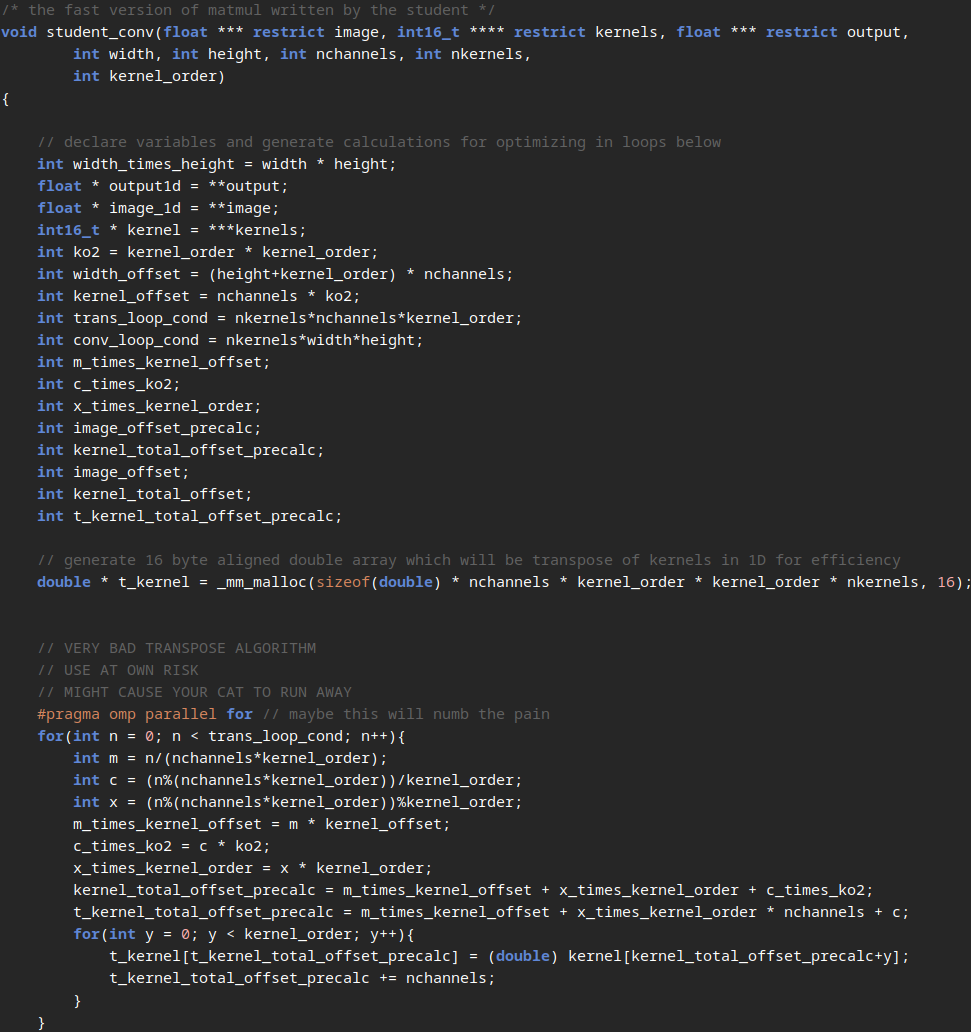
\includegraphics[width=0.65\textwidth]{images/student-conv-part1}
\end{frame}

\begin{frame}[fragile]
\frametitle{Continued: Source Code}
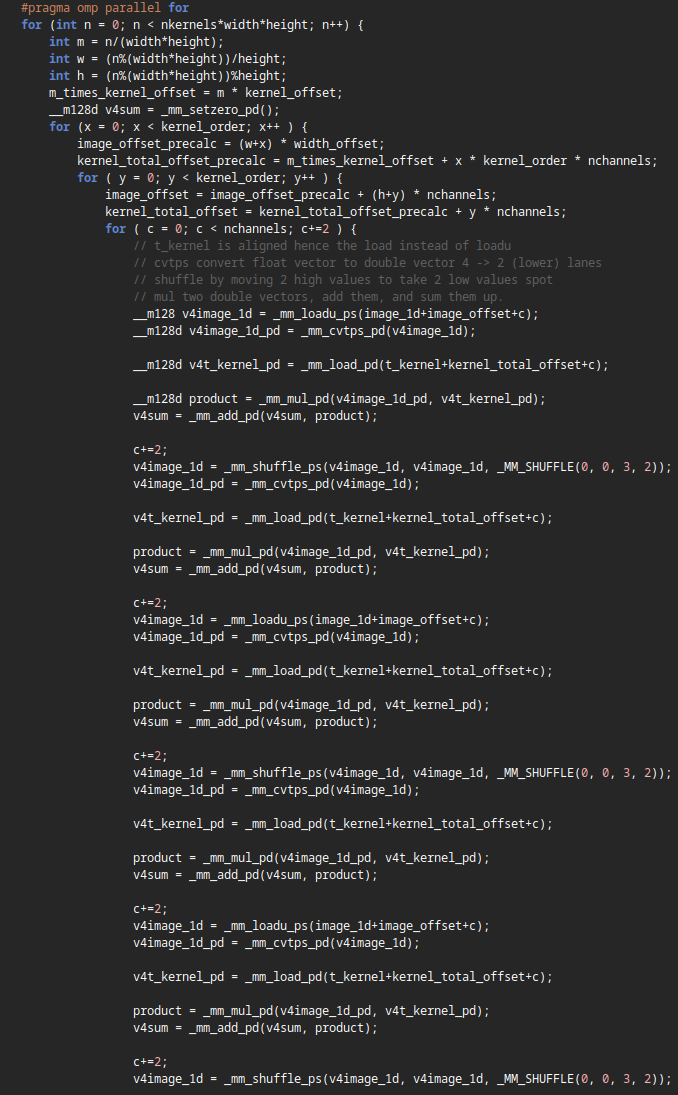
\includegraphics[width=0.4\textwidth]{images/student-conv-part2}
\end{frame}

\begin{frame}[fragile]
\frametitle{Continued: Source Code}
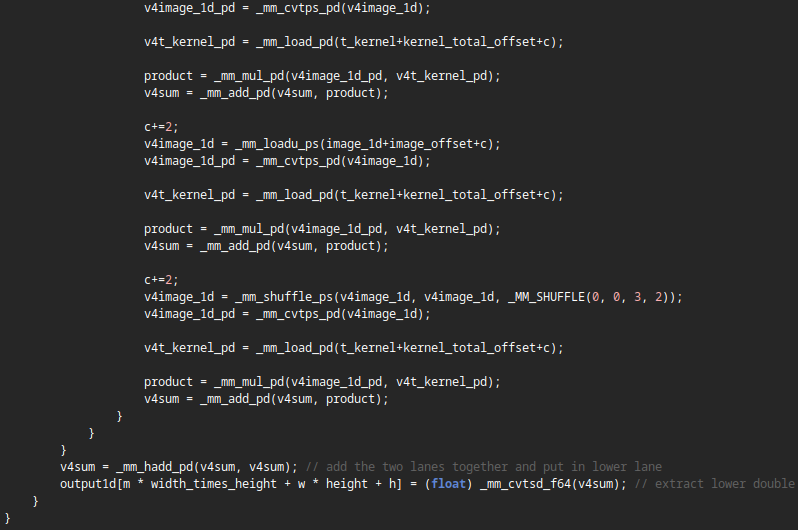
\includegraphics[width=1\textwidth]{images/student-conv-part3}
\end{frame}

\begin{frame}[fragile]
\frametitle{Speed Increase}
With test conv 128 128 7 256 256, we can get to nearly 90x speed increase. \\
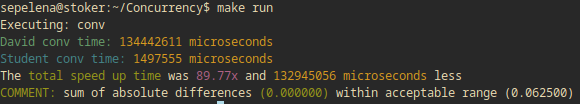
\includegraphics[width=1\textwidth]{images/stoker-89x}
\end{frame}

\begin{frame}[fragile]
\frametitle{Image Size and Speed Increase}
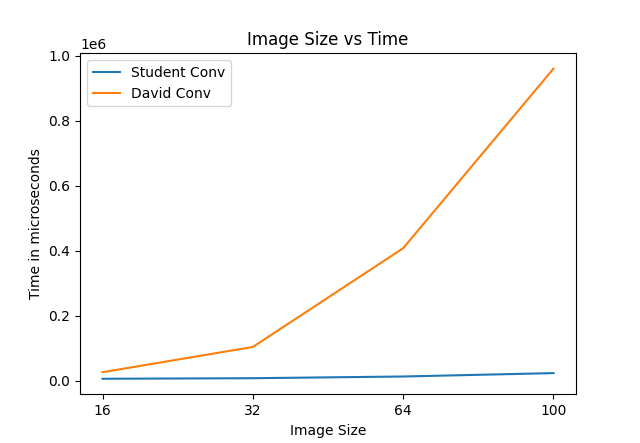
\includegraphics[width=1\textwidth]{images/Image_size_vs_time_X-X-5-32-32}
\end{frame}

\begin{frame}[fragile]
\frametitle{Image Size and Speed Increase}
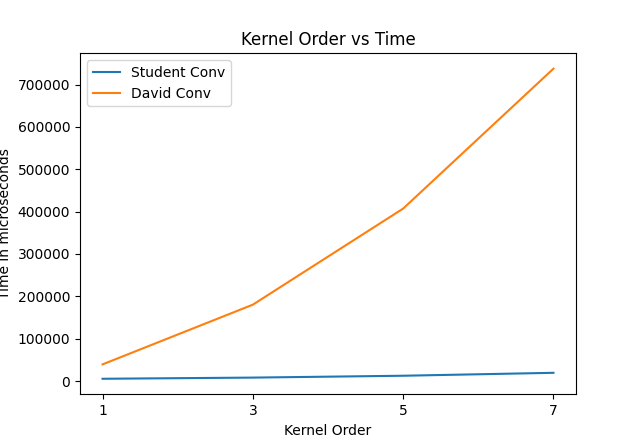
\includegraphics[width=1\textwidth]{images/kernel_vs_time_64-64-X-32-32}
\end{frame}

\begin{frame}[fragile]
\frametitle{Graphs}
%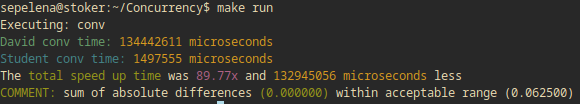
\includegraphics[width=1\textwidth]{images/stoker-89x}
\end{frame}

\end{document}
